% !TEX root= ...main.tex

\section{Функциональное назначение программы}

\subsection{Назначение программы}

%
\textbf{GIS Excelsior} предназначена для планирования колонизации планеты Марс. Под планированием подразумевается:

\begin{itemize}
	\item Выбор участка поверхности Марса для размещения колонии;
	\item Размещение зданий и модулей различного назначения на выбранном участке поверхности планеты с учетом соответствующих критериев размещения перечисленных в Таблице~\ref{tab:criterions}.
	\item Ознакомление с перечнем доступных для размещения объектов, их описанием и уровнями из таблицы критериев.
\end{itemize}
%



\subsection{Работа с интерфейсом}

%
При запуске сайта перед вами должен появиться следующий интерфейс:

\begin{figure}[h!]
	\centering
	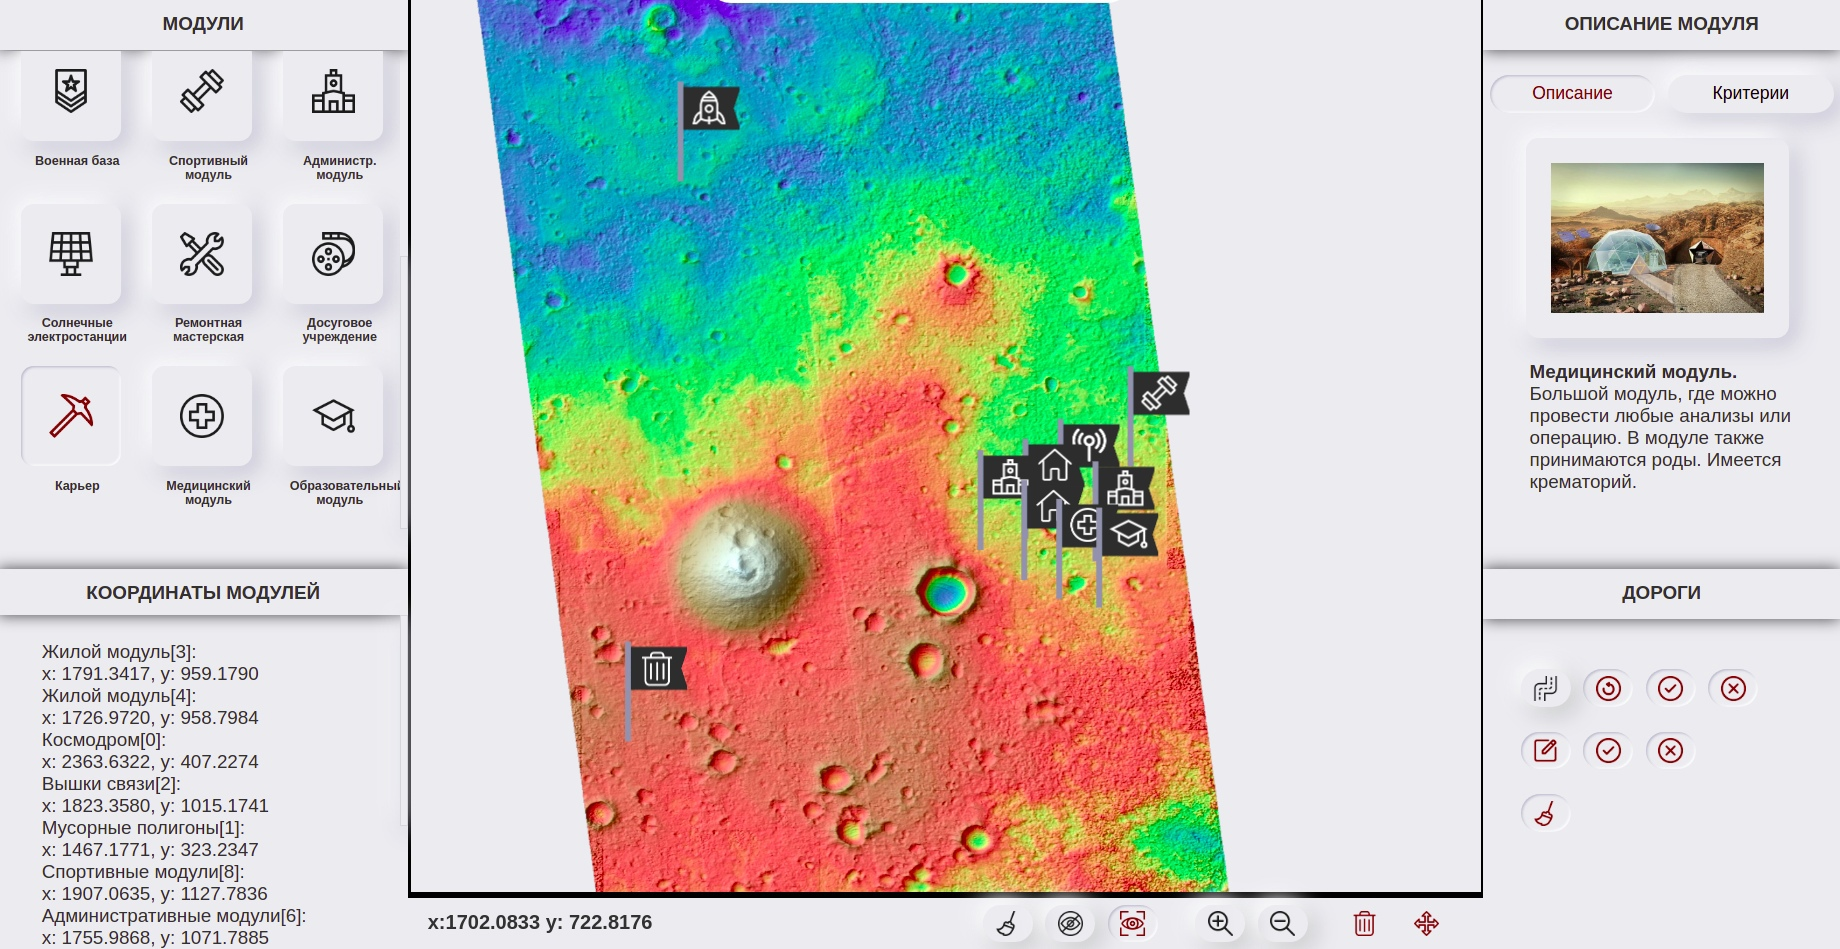
\includegraphics[width=.9\linewidth]{./img/interface}
	\caption{Общий вид интерфейса программы}\label{fig:interface}
\end{figure}

Самая главное, что вы должны видеть -- это участок поверхности Марса в \textbf{RGB} расцветке. Весь интерфейс можно разделить на 5 частей:

\begin{enumerate}
	\item \textbf{Центральная часть.} Здесь расположена карта,  инструменты для работы с размещенными на ней объектами, а также отображаются координаты точки под курсором.
	\item \textbf{Левый верхний угол.} Этот блок позволяет вам выбирать объект, который вы хотите разместить на карте.
	\item \textbf{Левый нижний угол.} Здесь будет появляться информация о размещенных объектах, их наименованиях и координаты.
	\item \textbf{Правый верхний угол.} В этом блоке вы можете заметить две вкладки: \textbf{<<Описание>>} и \textbf{<<Критерии>>}. Во вкладке <<Описание>> отображается фото с внешним видом выбранного объекта. Во вкладке <<Критерии>> написаны уровни критериев, которым соответствует выбранный объект.
	\item \textbf{Правый нижний угол.} В последнем блоке можно найти инструменты для размещения и редактирования дорог.
\end{enumerate}

Поговорим про каждый блок подробнее. В следующих параграфах.

\subsubsection*{Карта}

На карте вы можете разместить объекты из левого верхнего блока, а также "построить" дороги используя возможности правой нижней части интерфейса. Карта раскрашена в \textbf{RGB} расцветке по высотам. Высоты растут от синего цвета к красному и белому.

\begin{wrapfigure}{r}{.4\linewidth}
	\centering
	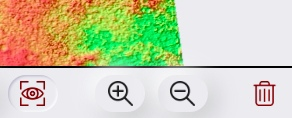
\includegraphics[width=.9\linewidth]{./img/zoom}
	\caption{Инструменты для изменения масштаба карты}\label{fig:zoom}
\end{wrapfigure}

Карту можно перемещать как вам удобно используя левую кнопку мыши (ЛКМ): наведите на карту, зажмите ЛКМ и перемещайте курсор не отпуская кнопку. Таким образом вы можете разместить нужный участок карты, например в центр.

Также можно использовать колесо мыши для приближения и отдаления (zoom) карты. Помимо этого вы можете кликать ЛКМ на соответствующие инструменты под картой, которые обозначены как две лупы (см.~рис.~\ref{fig:zoom}).

\begin{figure}[h!]
	\centering
	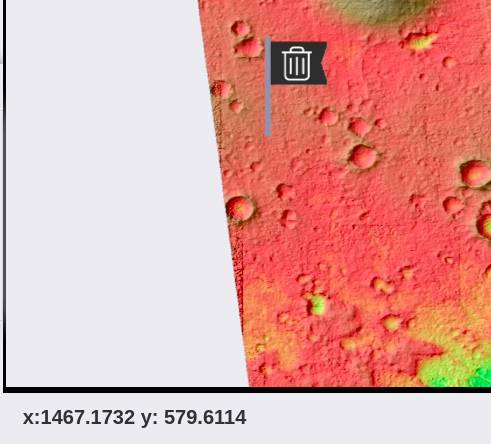
\includegraphics[width=.5\linewidth]{./img/coordinates}
	\caption{Отображение координат точки под курсором}\label{fig:coordinates}
\end{figure}

Можно заметить, что при наведении курсора на карту, в левом нижнем углу центрального окна видны координаты позиции (см.~рис.~\ref{fig:coordinates}). При перемещении курсора их можно отслеживать в реальном времени.

На панели инструментов под картой можно найти следующие инструменты: 

\begin{enumerate}
	\item \textbf{Очистить.} Очищает всю карту от любых объектов. \underline{Необратимое} действие.
	\item \textbf{Скрыть.} Скрывает все объекты карты, кроме дорог.
	\item \textbf{Показать.} Если какие-то объекты были скрыты, после нажатия этой кнопки они вернутся на карту.
	\item \textbf{Приблизить.} Уменьшает масштаб карты: все объекты становятся крупнее, а площадь обозреваемой поверхности уменьшается.
	\item \textbf{Отдалить.} Увеличивает масштаб карты: все объекты становятся меньше, а площадь обозреваемой поверхности увеличивается.
	\item \textbf{Удалить.} Удалить выбранный объект на карте. \underline{Необратимое} действие.
	\item \textbf{Переместить.} Переместить выбранный объект в другое место.
\end{enumerate}



%В нижней части центрального окна, вы можете увидеть несколько инструментов для работы с объектами на карте.
%
